\subsection{$n$D-Sphere-geodesic-line picking}
\label{sec:nsphere_geodesic_line}

Sphere-geodesic-line picking is similar to sphere-line picking, except
that the ``lines'' are geodesics on the surface of the sphere, and the
distance metric is the length of these lines.

Can we do this case in general ??? Yes we can all the way down to the circle which gives a uniform distribution.

$n$-Sphere is embedded in $\R^{n+1}$ and encloses the $n+1$-ball


Figures ...

\begin{figure}[tbp]
  \begin{center}
    \subfloat[\label{fig:sphere_geo_eg}Example.]
       {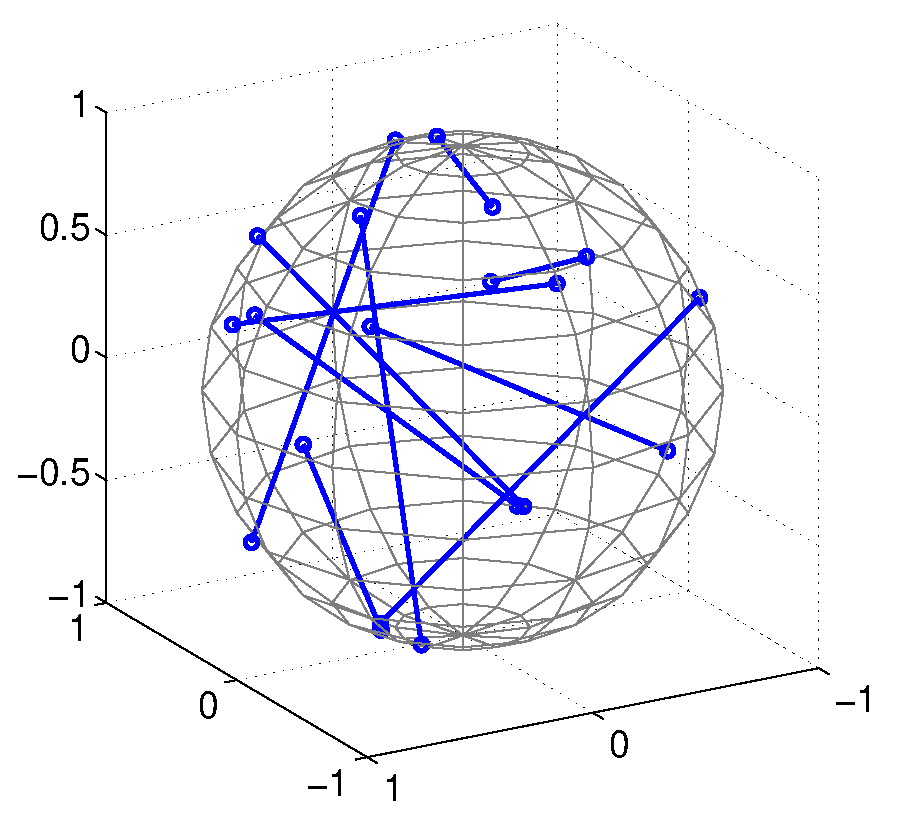
\includegraphics[width=0.4\columnwidth]{../Matlab/Plots/LinePicking_eg_sphere.eps}} 
    \hspace{6mm}
    \subfloat[\label{fig:sphere_geo_pdf}PDF.]
       {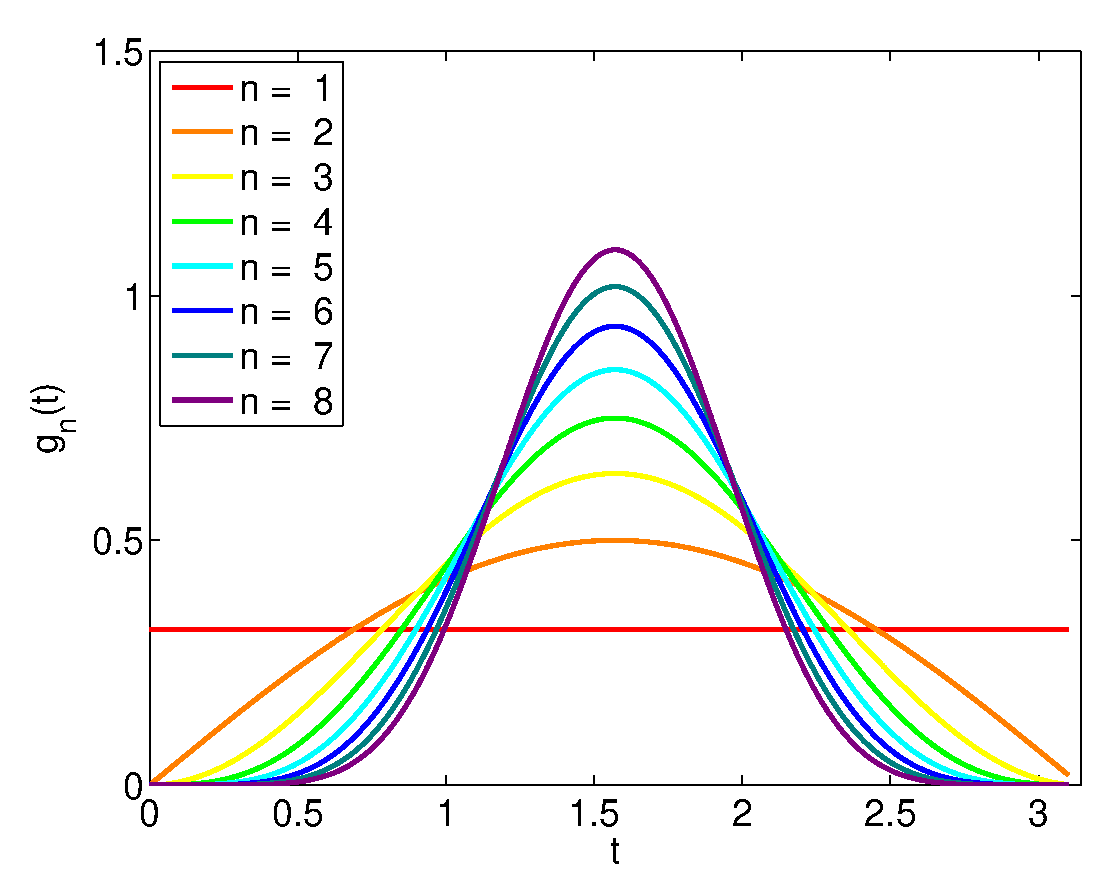
\includegraphics[width=0.48\columnwidth]{../Matlab/Plots/LinePicking_plot_nspheres_geodesic.eps}}
    \caption{The sphere-geodesic-line picking problem.}
  \end{center} 
\vspace{-4mm}
\end{figure}



\subsubsection{PDF}

Obviously, the sphere has spherical symmetry, but as a result, we can,
without loss of generality, assume the first point lies at the pole of
the sphere.

As in the $n$-Sphere above we first determine a density $f(\phi_1)$ function for $\phi_1$ then using the transform method. In fact $f(\phi_1)$ is exactly the same function as in the  $n$-Sphere thus we have:

\begin{equation}  
 f(\phi_1) = \frac{\Gamma\left(\frac{1+n}{2}\right) \sin(\phi )^{n - 1}}{\sqrt{\pi } \Gamma\left(\frac{n}{2}\right)}
\end{equation} 

We have have a function for $d$ the distance between two points in terms of $\phi_1$ so we can get  $\phi_1$ in terms of $d$ thus:

\begin{eqnarray}
  d & = & \phi_1  R.\\
\phi_1& = & \frac{d}{R}\\ 
   \frac {d \frac{d}{R}}{dd} & = & \frac{1}{R}\\
\end{eqnarray}



If $y = g(X)$ then the transform rule  is :  

\[ f_Y(y) = \left| \frac{d}{dy} \left( g^{-1}(y) \right) \right|
                f_X\left( g^{-1}(y) \right)
\]

thus 
\begin{eqnarray}
g_{R}^{n}(d) & = &  \left|\frac{1}{R}\right|  f\left(\frac{d}{R} \right)\\
            & = &   \frac{\Gamma\left(\frac{1+n}{2}\right) 
                            \sin\left(\frac{d}{R}\right)^{n-1}}
                        {\sqrt{\pi } R \Gamma\left(\frac{n}{2}\right)}
\end{eqnarray}

\subsubsection{CDF}
\begin{equation}
G_{R}^{n}(d)=\frac{1}{2}-\frac{\cos\left(\frac{d}{R}\right) \sin\left(\frac{d}{R}\right)^n \left(\sin\left(\frac{d}{R}\right)^2\right)^{-n/2}\Gamma\left(\frac{1+n}{2}\right) {}_{2}F_{1}\left(\frac{1}{2},1-\frac{n}{2},\frac{3}{2},\cos\left(\frac{d}{R}\right)^2\right) }  {\sqrt{\pi } \Gamma\left(\frac{n}{2}\right)}
\end{equation}

\subsubsection{Moments}

\begin{equation}
E[g_{R}^{n}(d)]=\frac{\pi R}{2}
\end{equation}

The mean can be derived either by symmetry (noting that PDF is symmetric around
$t = \pi R/2$, or directly using \cite[3.821,1.(p.446)]{GandR}
\begin{equation}
  \label{eq:sin_x_x}
  \int_0^\pi x \sin^p x \, dx =
       \frac{\pi^2}{2^{p+1}} \, \frac{\Gamma(p+1)}{ \Gamma\left(p/2+1 \right)^2 }, \mbox{ for } p>-1.
\end{equation}
The result is 
\begin{eqnarray}
  \label{eq:mean_nsphere_geo}
 E[X] & = & \int_0^{\pi R} 
                    s g_{R}^{n}(s)
                   \, ds \nonumber \\
      & = & \frac{\Gamma\left(\frac{1+n}{2}\right) }
                        {\sqrt{\pi } R \Gamma\left(\frac{n}{2}\right)}
            \int_0^{\pi R} 
                    s  \sin \left( \frac{s}{R} \right)^{n-1}
                   \, ds \nonumber \\
      & = & \frac{\Gamma\left(\frac{1+n}{2}\right) }
                        {\sqrt{\pi } \Gamma\left(\frac{n}{2}\right)}
            \int_0^{\pi R} 
                    (R u)  \sin \left( u \right)^{n-1}
                   \, ds \nonumber \\
      & = & \frac{R \Gamma\left(\frac{1+n}{2}\right) }
                        {\sqrt{\pi } \Gamma\left(\frac{n}{2}\right)}
            \int_0^{\pi R} 
                    u \sin \left( u \right)^{n-1}
                   \, ds \nonumber \\
      & = & \frac{R \Gamma\left(\frac{1+n}{2}\right) }
                        {\sqrt{\pi } \Gamma\left(\frac{n}{2}\right)}
                \frac{\pi^2}{2^{n}} \, \frac{\Gamma(n)}{ \Gamma\left((n-1)/2-1 \right)^2 }
             \nonumber \\
       & = & \nonumber \\
       & = & \frac{\pi R}{2}.
\end{eqnarray}

Higher order moments are harder: possible approaches:

-- $n=2$ can use twice angle formula
\[
\sin^2 x = 1 - \cos^2 x = 1 - ( \cos 2 x +1)/2 = (1 - \cos 2x )/2 .
\]
and \cite[3.761 (p.421)]{GandR}, which gives various combinations
of powers and trig functions.

-- Fourier convolution, but don't know Fourier for higher powers of sin

-- power series of $sin^n$
\begin{equation}
  \label{eq:sin^n_taylor}
  \sin^{n-1}(x) = 
\end{equation}

-- expansion of $sin^n$ as a binomial of $exp$
\begin{equation}
  \label{eq:sin^n_taylor}
  \sin^{n-1}(x) = \left[ \frac{e^{i x} - e^{-i x} }{2 i} \right]^{n-1}
\end{equation}

-- or maybe?

\[ \Gamma(s) \Gamma(1-s) = \frac{\pi}{\sin \pi s} \]


Take $R=1$, then $t \in [0, \pi$ and 
\begin{eqnarray}
g_{R}^{n}(t) & = &   \frac{\Gamma\left(\frac{1+n}{2}\right) }
                         {\sqrt{\pi } R\Gamma\left(\frac{n}{2}\right)}  
                      \sin(t)^{n-1} \nonumber \\
   & = &   \frac{\Gamma\left(\frac{1+n}{2}\right) }
                {\sqrt{\pi } R\Gamma\left(\frac{n}{2}\right)}  
                      \sin(t)^{n-1} \nonumber \\
\end{eqnarray}


